\subsection*{3.4 Durchflutungsgesetz}
    \begin{minipage}{0.64\linewidth}
        \begin{empheq}[box = \fbox]{align*}
            \begin{array}{r@{\ }l} %{r@{\ }c@{\ }l}
                \oint\limits \vec{H} ds &= n \cdot I_{tot}\\
                &= \int \vec{j} + \frac{\vec{dD}}{dt} \vec{dA}\\
                rot(\vec{H}) &= \vec{j} + \dot{\vec{D}}
            \end{array}
        \end{empheq}  
    \end{minipage}
    \begin{minipage}{0.34\linewidth}
        \begin{scriptsize}
            \begin{empheq}{align*}
                \vec{H} &= \text{mag. Feldstärke}\\
                I &= j \cdot A = \text{el. Strom}\\
                j &= \text{Stromflächendichte}\\
                D &= \text{el. Flussdichte}
            \end{empheq}
        \end{scriptsize}
    \end{minipage}

    \subsubsection{Feldstärke eines geradlinigen Leiters}
        \begin{minipage}{0.34\linewidth}
            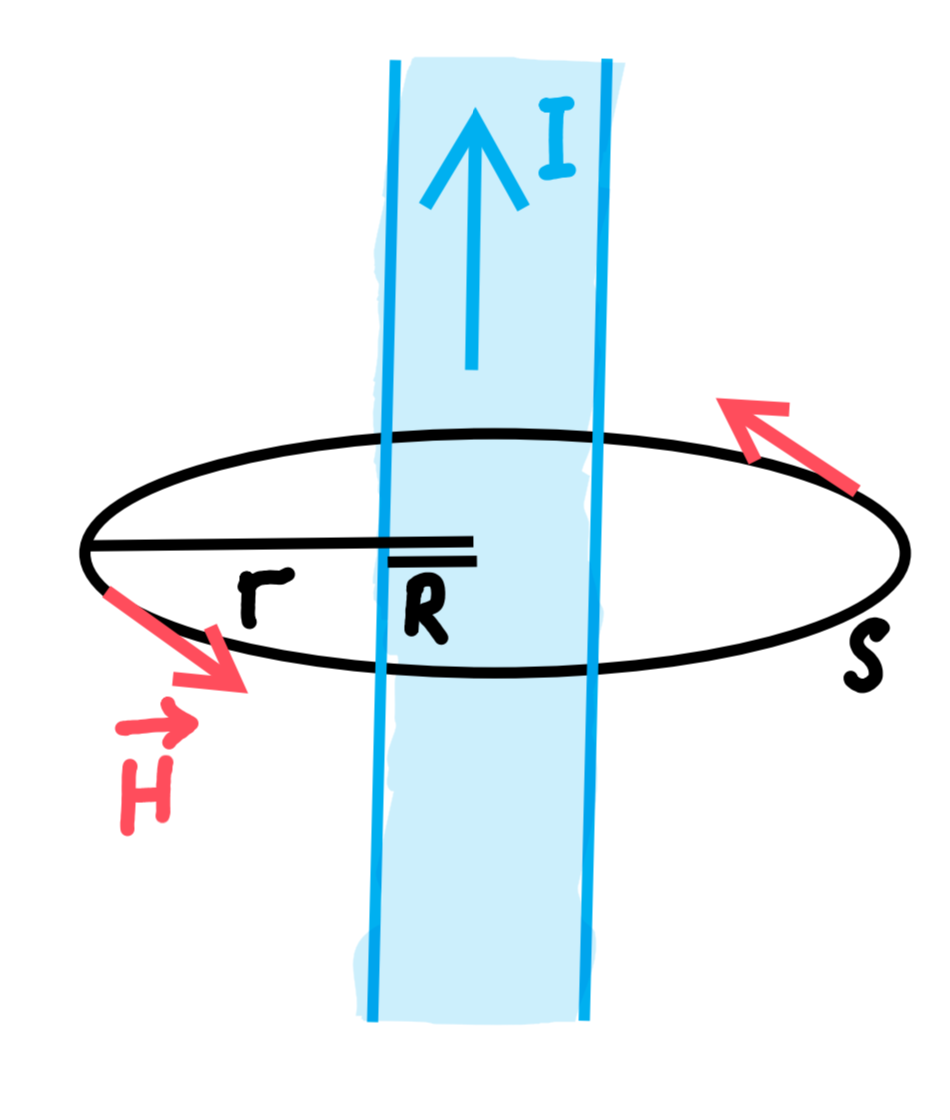
\includegraphics[width = \linewidth]{src/images/mag-feld_gerader_leiter.png}
        \end{minipage}
        \begin{minipage}{0.64\linewidth}
            Durchflutungsgesetz führt zu:
            \begin{empheq}[box = \fbox]{align*}
                \text{In Leiter: } H(r) &= \frac{I}{2 \pi} \frac{r}{R^2}\\
                \text{Um Leiter: } H(r) &= \frac{I}{2 \pi r}
            \end{empheq}
            \begin{scriptsize}
                \begin{empheq}{align*}
                    H &= \text{mag. Feldstärke}\\
                    I &= \text{el. Strom}\\
                    R &= \text{Radius des el. Leiters}\\
                \end{empheq}
            \end{scriptsize}
        \end{minipage}